 \chapter{La détection d'objets}
\minitoc
\newpage
\pagestyle{fancy}
\fancyhead[L]{\chaptername \ \thechapter}
\fancyhead[R]{La détection d'objets}
\renewcommand{\headrulewidth}{1pt}
\fancyfoot[C]{\thepage}

\section{Introduction} 
La vision par ordinateur est actuellement l'un des domaines les plus actifs de l'intelligence artificielle, et la détection d'objets a joué un rôle clé dans son développement rapide. 
Le besoin de détection d'objets est d'automatiser les tâches difficiles qui nécessitent une intervention humaine ou impossible à faire par l'homme. Par exemple, la tâche de lire le numéro d'immatriculation de chaque voiture qui passe sur l'autoroute où les voitures passent à grande vitesse que l'œil humain avec le cerveau est incapable de percevoir quelques chiffres, sans parler du numéro d'enregistrement complet.

L'objectif principal de ce chapitre est de comprendre les concepts de base de la détection d'objets.

\section{Définition}
La détection d'objets est une technique de vision par ordinateur qui permet d'identifier et de localiser des objets dans une image ou une vidéo. Plus précisément, la détection d'objet dessine des cadres de délimitation autour de ces objets détectés, ce qui nous permet de localiser où se trouvent  objets (ou comment ils se déplacent) dans une scène donnée. 

Donc,  la boîte englobante de détection d'objet(généralement un carré ou un rectangle) constitue le composant clé  qui identifie les bords de l'objet étiqueté. Elle est accompagnée d'une étiquette de l'objet, qu'il s'agisse d'une personne, d'une voiture ou d'un autre objet pour décrire l'objet cible. Les boîtes englobantes peuvent se chevaucher pour présenter plusieurs objets dans un plan donné tant que le modèle a une connaissance préalable des éléments qu'il étiquette.

\section{Détection d'objets vs. Autres tâches de vision par ordinateur}
Avant de plonger dans les applications de détection d'objets, les cas d'utilisation et les méthodes de détection d'objets de base, il est crucial d'établir une compréhension claire de la détection d'objets elle-même. Le terme est souvent utilisé de manière interchangeable avec des techniques telles que la classification d'images, la reconnaissance d'objets, la segmentation, etc. Cependant, il faut reconnaître que bon nombre de celles mentionnées ci-dessus sont des tâches distinctes qui relèvent généralement de la détection d'objets. Il est inexact de les utiliser comme synonymes les uns des autres puisque chacun se rapporte à une tâche tout aussi vitale.
Ainsi, nous pouvons distinguer ces trois tâches de vision par ordinateur :

\begin{enumerate}
\item \underline{\textbf{Classification d'images:}}
Il s'agit de prédire la classe d'un élément dans une image. 
    
\begin{itemize}
\item \textbf{Entrée : }une image avec un seul objet, comme une photographie.
         
\item \textbf{Sortie :} une étiquette de classe 
\end{itemize}

\item \underline{\textbf{Localisation d'objets}}
Il s'agit de localiser la présence d'objets dans une image et indiquer leur emplacement à l'aide d'un cadre de délimitation (voir figure \ref{im4}.
     
\begin{itemize}
\item  \textbf{Entrée :} Une image avec un ou plusieurs objets, comme une photographie.
\item  \textbf{Sortie :} une ou plusieurs boîtes englobantes (par exemple définies par un point, une largeur et une hauteur).
\end{itemize}

\begin{figure}[H]
\centering
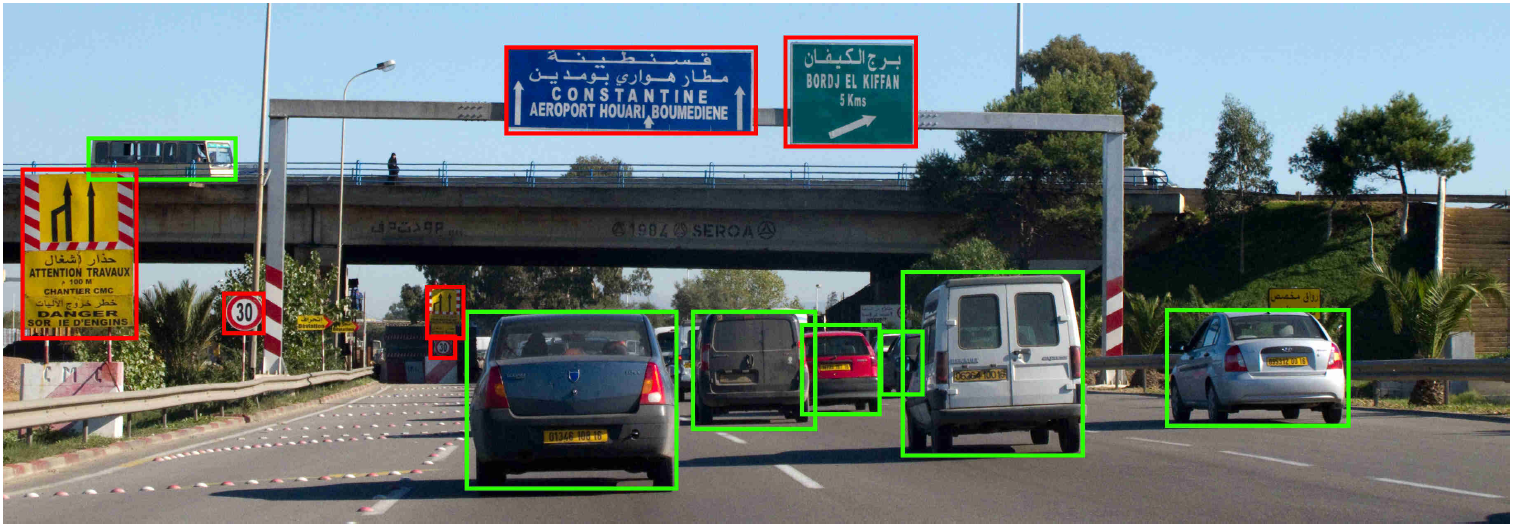
\includegraphics[height=5.7cm,width=16cm]{Chapitre1/im4.png}
\caption{Localisation d'objets.}
\label{im4}
\end{figure}

\item \underline{\textbf{Détection d'objets :}}
Il s'agit de localiser la présence d'objets avec une boîte englobante et les types ou classes d'objets localisés dans une image. 

\begin{itemize}
\item  \textbf{Entrée : }Une image avec un ou plusieurs objets, comme une photographie.
\item \textbf{Sortie :} une ou plusieurs boîtes englobantes (par exemple définies par un point, une largeur et une hauteur) et une étiquette de classe pour chaque boîte englobante.   
 \end{itemize}
 La figure \ref{im7} montre clairement un résultat d'un processus de détection d'objets dans une scène routière

\begin{figure}[H]
\centering
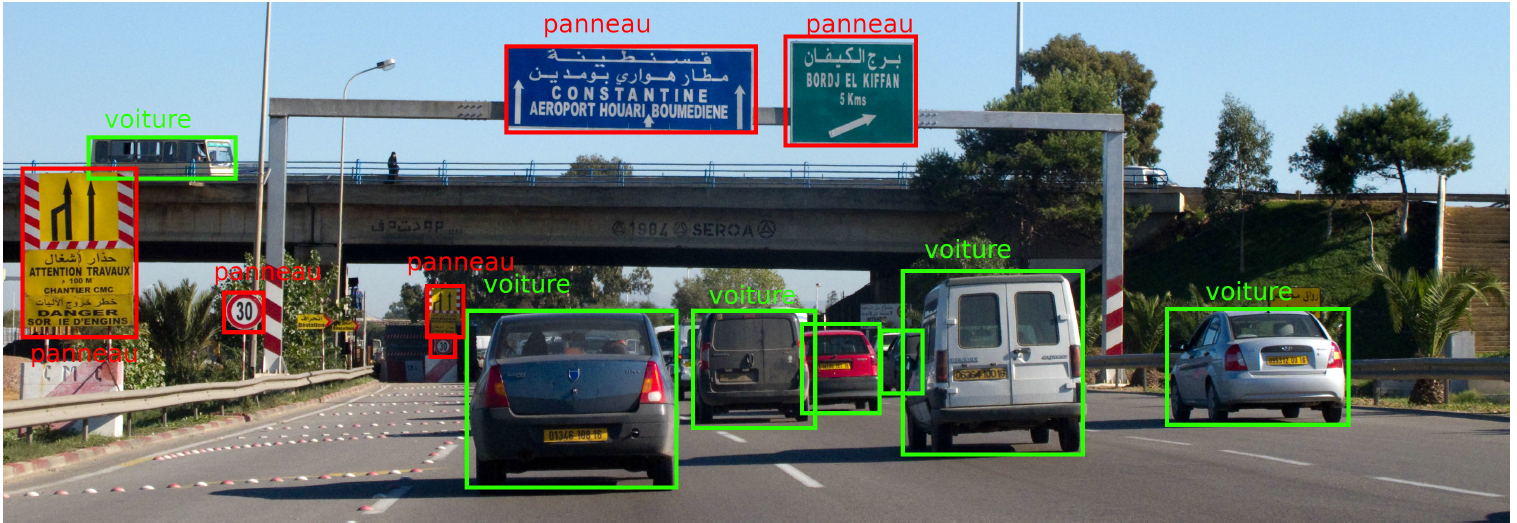
\includegraphics[height=7cm,width=16cm]{Chapitre1/im7.png}
\caption {Détection d'objets.}
\label{im7}
\end{figure}
     
La technique de la boîte englobante est la méthode traditionnelle d'étiquetage des données dans l'image. Les cadres de délimitation sont des marqueurs d'annotation dessinés autour des objets dans une image. Contours mais en forme rectangulaire. 
\end{enumerate}

Une autre extension de cette répartition des tâches de vision par ordinateur est \underline{\textbf{la segmentation sémantique}}  des images où les instances d'objets reconnus sont indiquées en mettant en évidence les pixels spécifiques de l'objet,  sans limiter l'objet d'un cadre de délimitation.  Cette technique donne un emplacement précis (au niveau du pixel) d'un objet et des pixels trouvés. les pixels produits peuvent aussi être appelés: masque.
(voir figure \ref{im5}.


\begin{figure}[H]
\centering
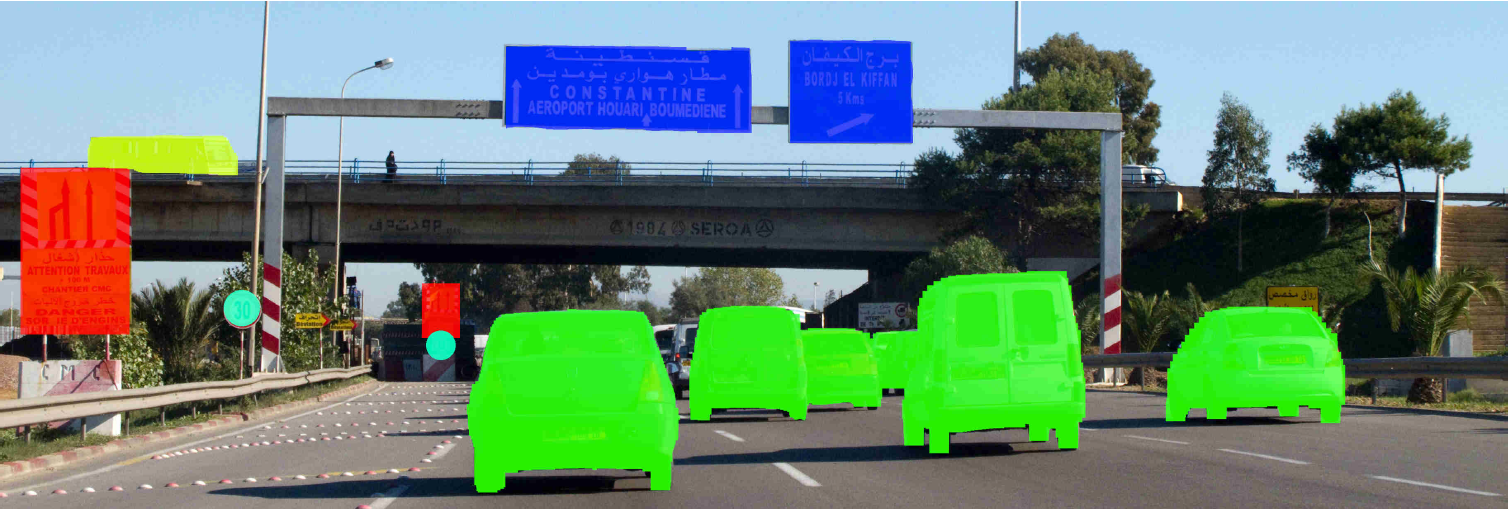
\includegraphics[height=5.7cm,width=16cm]{Chapitre1/im5.png}
\caption{Segmentation sémantique.}
\label{im5}
\end{figure}

La combinaison de la segmentation sémantique avec la détection d'objets conduit à la \underline{\textbf{segmentation d'instance}}, qui détecte d'abord les instances d'objet, puis segmente chacune dans les boîtes détectées (appelées dans ce cas régions d'intérêt). En d'autre termes, chaque objet de l'image obtient son masque unique même s'il existe d'autres objets avec la même classe (voir figure .    

\begin{figure}[H]
\centering
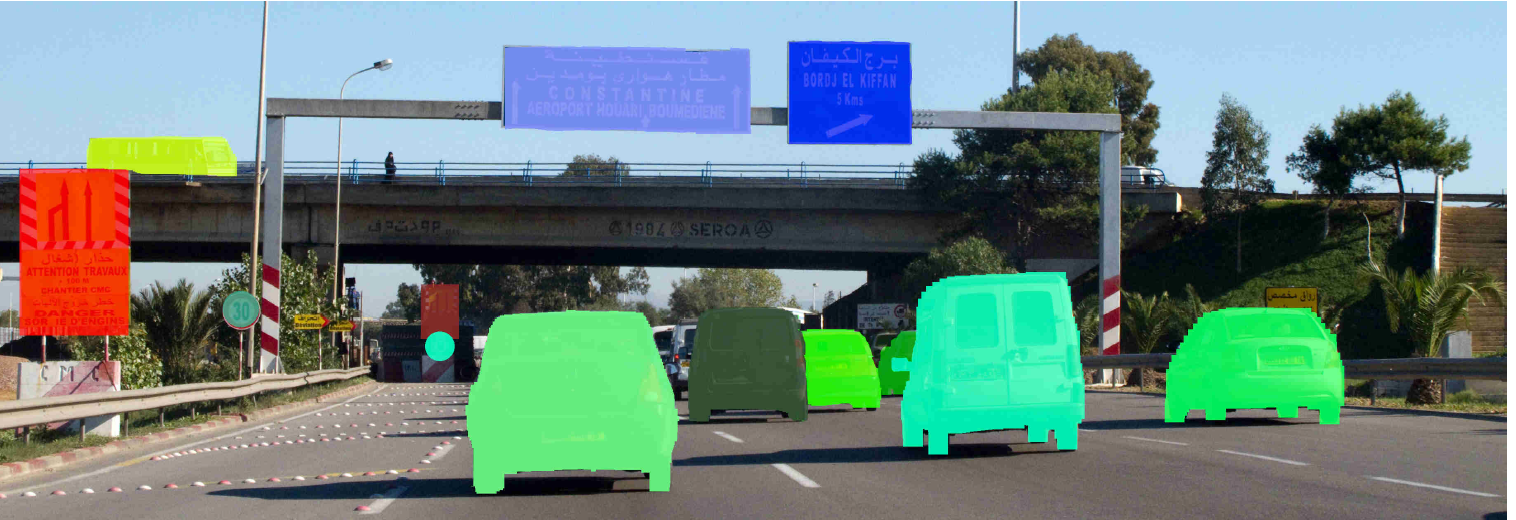
\includegraphics[height=5.7cm,width=16cm]{Chapitre1/im6.png}
\caption{Segmentation par instance.}
\label{im6}
\end{figure}     


% =========== Apps ===========
\section{Les applications de la détection d'objets}
La détection et la reconnaissance d'objets sont appliquées dans de nombreux domaines de la vision par ordinateur, notamment la récupération d'images, la sécurité, la surveillance, les systèmes de véhicules automatisés et l'inspection des machines. La détection d'objets fait son entrée dans un large éventail d'industries, avec des cas d'utilisation allant de la sécurité personnelle à la productivité sur le lieu de travail.

Dans cette section, nous discutons  certaines applications actuelles  des systèmes de détection d'objets dans divers domaines:
     % =========== OCR ===========
     \subsection{Reconnaissance optique de caractères }
La reconnaissance optique de caractères, souvent abrégé en OCR, est la conversion d'images de texte  manuscrit ou imprimé en texte codé par machine, qu'il s'agisse d'un document numérisé, d'une photo d'un document, d'une scène-photo (par exemple le texte sur des panneaux  publicitaires dans une photo de paysage) ou à partir d'un texte de sous-titre superposé à une image (voir figure \ref{ocr}).
\begin{figure}[H]
\centering
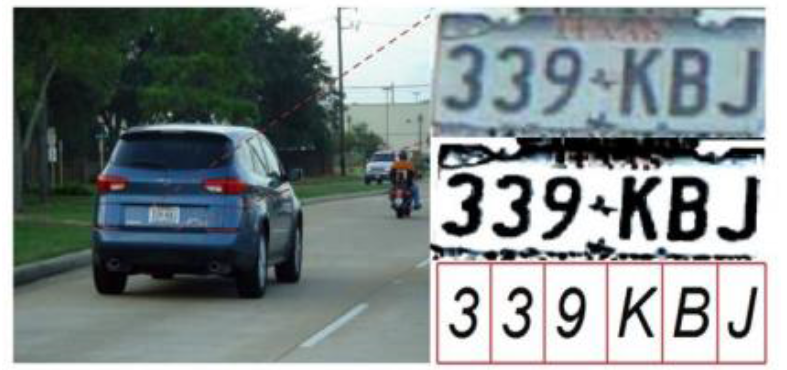
\includegraphics[height=5cm,width=12.5cm]{Chapitre1/ocr.png}
\caption{Reconnaissance optique de caractères.}
\label{ocr}
\end{figure}     
Largement utilisé comme forme de saisie d'informations à partir d'enregistrements de données papier imprimés - qu'il s'agisse de documents de passeport, de factures, de relevés bancaires, de reçus informatisés, de cartes de visite, de courrier, d'impressions de données statiques ou de toute documentation appropriée, il s'agit d'une méthode courante de numérisation des textes imprimés afin qu'ils puissent être numérisés, recherchés, stockés de manière plus compacte, affichés en ligne et utilisés dans des processus automatiques tels que la traduction automatique, la synthèse vocale,  etc.
     
     % =========== Self-Driving ===========
     \subsection{Voitures autonomes}
 L'un des meilleurs exemples de la raison pour laquelle la détection d'objets est très nécessaire est la conduite autonome. Pour qu'une voiture décide quoi faire à l'étape suivante, que ce soit accélérer, freiner ou tourner, elle doit savoir où se trouvent tous les objets autour de la voiture et quels sont ces objets.  Cela nécessite la détection d'objets pour entraîner essentiellement la voiture à détecter un ensemble connu d'objets tels que des voitures, des piétons, des feux de circulation, des panneaux de signalisation, des vélos, des motos, etc.

      \begin{figure}[H]
          \centering
          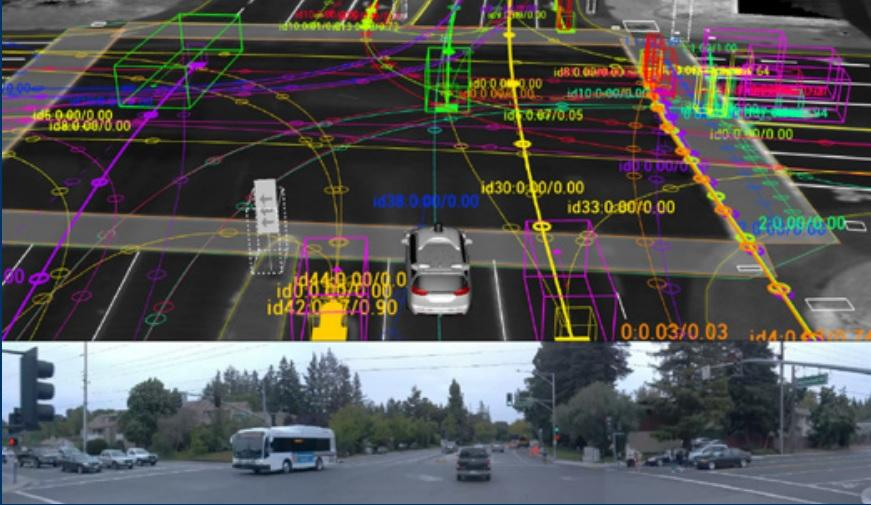
\includegraphics[height=7cm,width=12cm]{Chapitre1/img12.jpg}
          \caption{carte de l'environnement des voitures autonomes générée à l'aide de la détection d'objets.}
          \label{img12}
          \end{figure}
\subsection{Suivi des objets}
Le système de détection d'objets est également utilisé pour suivre les objets, par exemple suivre un ballon pendant un match de football, suivre une personne dans une vidéo. Le suivi d'objets a une variété d'utilisations, dont certaines sont la surveillance et la sécurité , surveillance du trafic, communication vidéo, vision et animation de robots.

Après avoir découvert ces objets, on a parfois envie de les suivre. Le suivi consiste à suivre un objet dans une vidéo. En gros, dès qu'un des objets est détecté, un identifiant lui est attribué et suivi jusqu'à ce qu'il ne soit plus visible sur l'image.

La figure \ref{so} montre un exemple pour mieux comprendre de quoi il s'agit, malgré qu'on parle de suivi lorsqu'il s'agit d'une vidéo).

\begin{figure}[H]
\centering
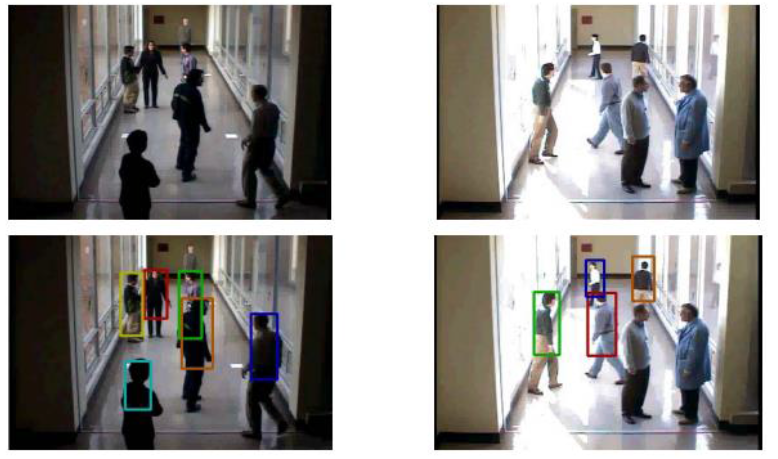
\includegraphics[height=6.5cm,width=13cm]{Chapitre1/so.png}
\caption{Suivi d'individus.}
\label{so}
\end{figure}     
     % =========== Biometrics ===========
     \subsection{Biométrie}
       
     L'authentification par vérification biométrique est de plus en plus courante dans les systèmes de sécurité d'entreprise et publics,  et les applications de point de vente. Certaines méthodes biométriques, telles que la reconnaissance faciale et la reconnaissance de l'iris, sont fortement basées sur la détection d'objets.
     \begin{figure}[H]
          \centering
          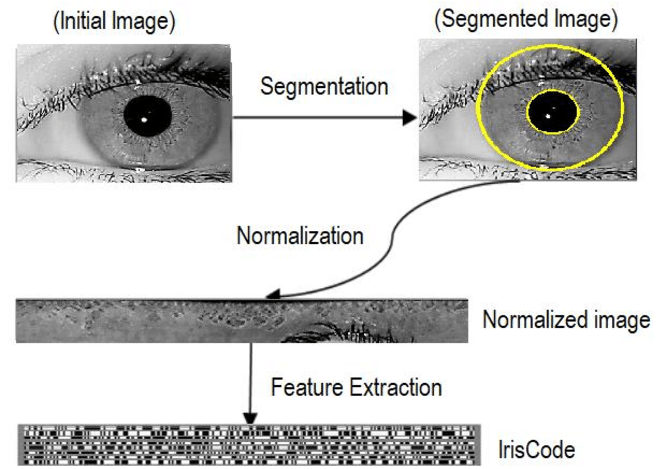
\includegraphics[height=7cm,width=12cm]{Chapitre1/img13.png}
          \caption{Identification de l'iris à l'aide de la détection d'objet.}
          \label{img13}
          \end{figure}
     
     % =========== Acitivity ===========
     \subsection{Reconnaissance d'activités}
     La reconnaissance d'activité vise à reconnaître les actions et objectifs d'un ou plusieurs agents à partir d'une série d'observations sur les actions des agents et les conditions environnementales. Ce domaine de recherche a attiré l'attention de plusieurs communautés informatiques en raison de sa capacité à fournir un support personnalisé pour de nombreuses applications différentes et de sa connexion à de nombreux domaines d'études différents tels que l'interaction homme-machine ou la sociologie.
     \begin{figure}[H]
          \centering
          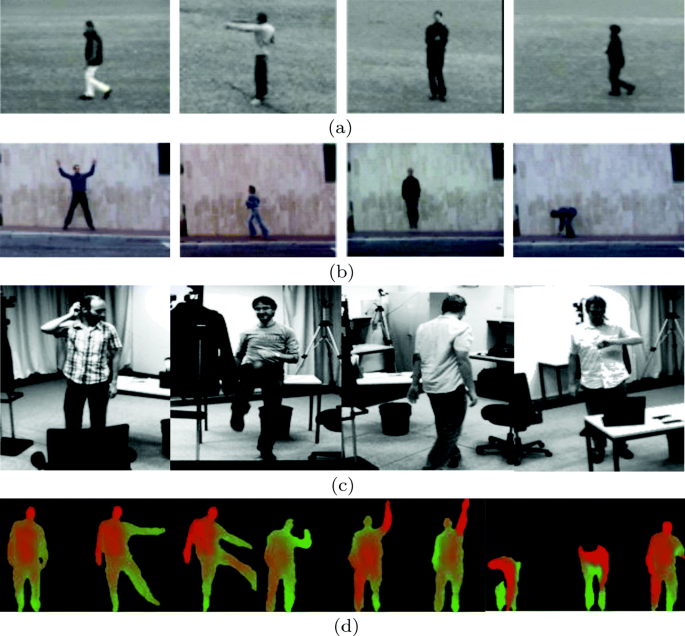
\includegraphics[height=10cm,width=12cm]{Chapitre1/img14.png}
          \caption{Reconnaissance d'activités.}
          \label{img14}
          \end{figure}

     % =========== Med ===========
     \subsection{Imagerie médicale}
     Les outils de traitement d'images médicales jouent un rôle de plus en plus important pour aider les médecins et les spécialistes dans le diagnostic, la planification thérapeutique et les interventions guidées par l'image. Le suivi précis, robuste et rapide d'objets anatomiques déformables tels que le cœur est une tâche cruciale dans l'analyse d'images médicales.
     \begin{figure}[H]
          \centering
          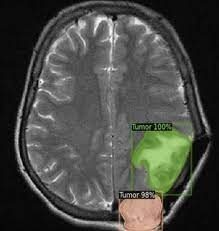
\includegraphics[height=6cm,width=6cm]{Chapitre1/img15.jpg}
          \caption{Détection de tumeurs cérébrales à l'aide de méthodes de détection d'objets.}
          \label{img15}
          \end{figure}

     % =========== Robo ===========
     \subsection{Robotique}
     Les robots d'assistance autonomes doivent être dotés de la capacité de traiter les données visuelles en temps réel afin qu'ils puissent réagir de manière adéquate pour s'adapter rapidement aux changements de l'environnement. La détection et la reconnaissance fiables d'objets sont généralement une première étape nécessaire pour atteindre cet objectif.
     \begin{figure}[H]
          \centering
          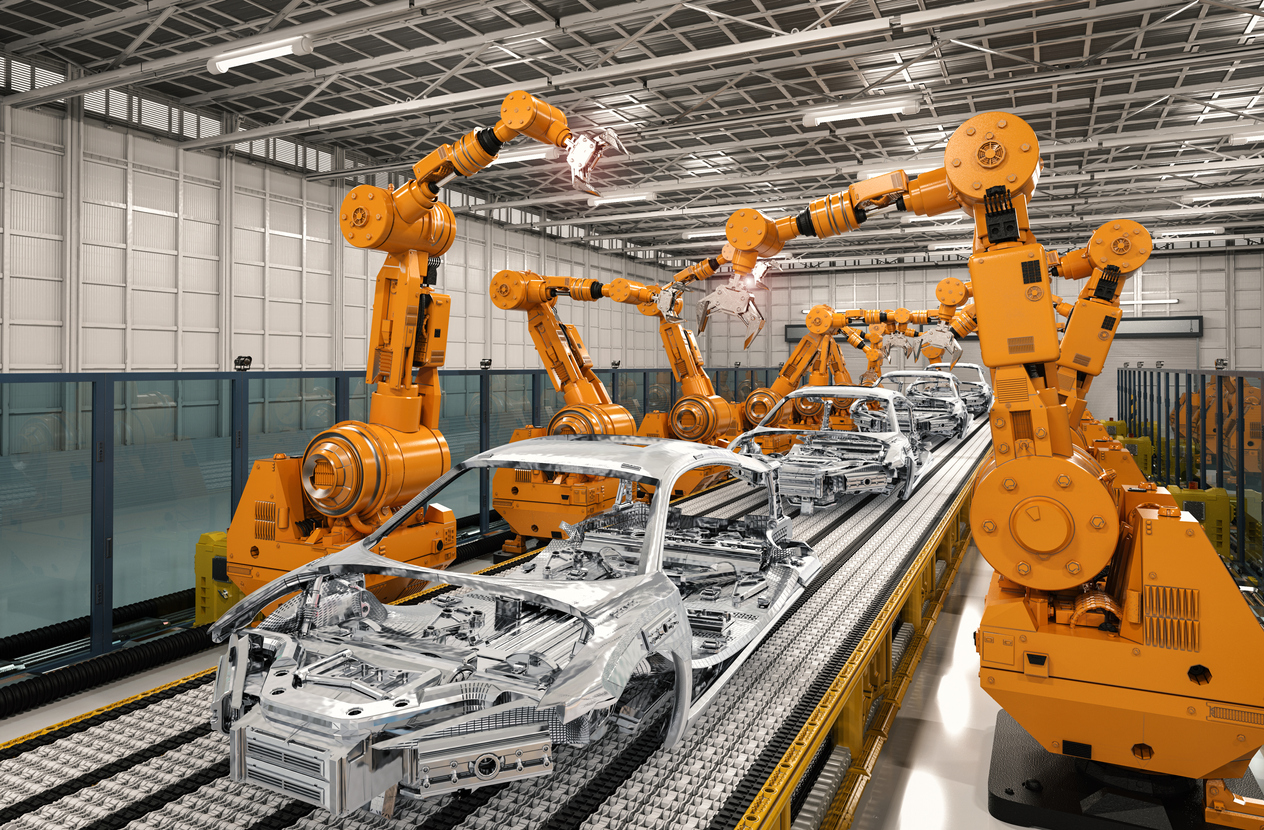
\includegraphics[height=6cm,width=10cm]{Chapitre1/img16.jpg}
          \caption{Mains robotiques utilisées dans la construction automobile.}
          \label{img16}
          \end{figure}
     
     % =========== Factory ===========
     \subsection{Production industrielle}
     Les usines du monde entier s'efforcent de produire des produits de la meilleure qualité avec un coût de production minimum. Cependant, pour  atteindre cet objectif, les usines doivent embaucher de la main-d'œuvre pour vérifier la qualité des composants, ce qui augmente le coût de production et d'autres problèmes liés au travail manuel, comme la dextérité et la productivité du travailleur. La détection d'objets résout les problèmes liés au travail manuel, elle garantit que les bons composants sont utilisés dans les chaînes de montage et que les processus corrects sont suivis avec une précision et une exactitude élevées, plus qu'un travail manuel et à moindre coût.
     \begin{figure}[H]
          \centering
          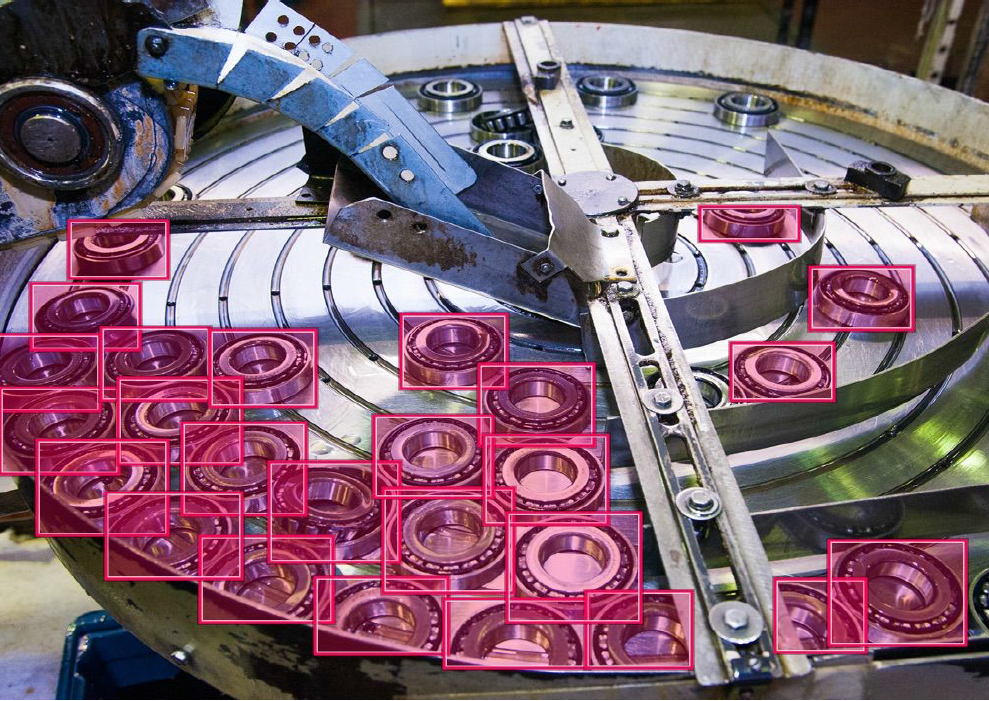
\includegraphics[height=6cm,width=11cm]{Chapitre1/im8.png}
          \caption{Détection d'objets utilisée pour détecter les pièces fabriquées mal formées.}
          \label{im8}
          \end{figure}
     
     
     % =========== Security ===========
     \subsection{Surveillance et sécurité}
     Dans les grandes villes où la population est très élevée, dans les zones industrielles, les grandes banques et de nombreuses autres zones hautement sensibles, la sécurité est indispensable 24 heures sur 24 et il est presque impossible pour un être humain d'atteindre ce niveau. La détection d'objets est donc une solution à ce type de problèmes où elle suit les mouvements des visiteurs, suit les comportements des individus ou des véhicules, fait la distinction entre les activités autorisées et non autorisées et signale lorsqu'un objet inattendu nécessite une enquête. tout cela 24 heures sur 24 sans arrêt et aussi à moindre coût de maintenance.
     \begin{figure}[H]
          \centering
          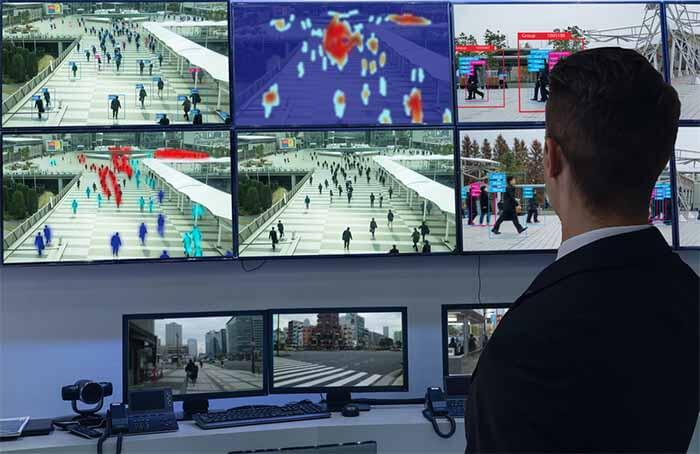
\includegraphics[height=6cm,width=12cm]{Chapitre1/img17.jpeg}
          \caption{Détection d'objets utilisée dans la sécurité et la surveillance.}
          \label{im17}
          \end{figure}

     % =========== Recherche visuelle ===========
     \subsection{Recherche d'images}   
     Puisqu'une image peut contenir des dizaines d'objets, la détection d'objets rend aussi simple que possible la recherche d'image. De la même manière que la saisie semi-automatique améliore l'expérience de recherche de texte, la détection d'objets fait de la recherche visuelle une expérience plus fluide. La détection d'objets dans la recherche visuelle permet également de nouvelles fonctionnalités, telles que la correspondance d'objet à objet.
     \begin{figure}[H]
          \centering
          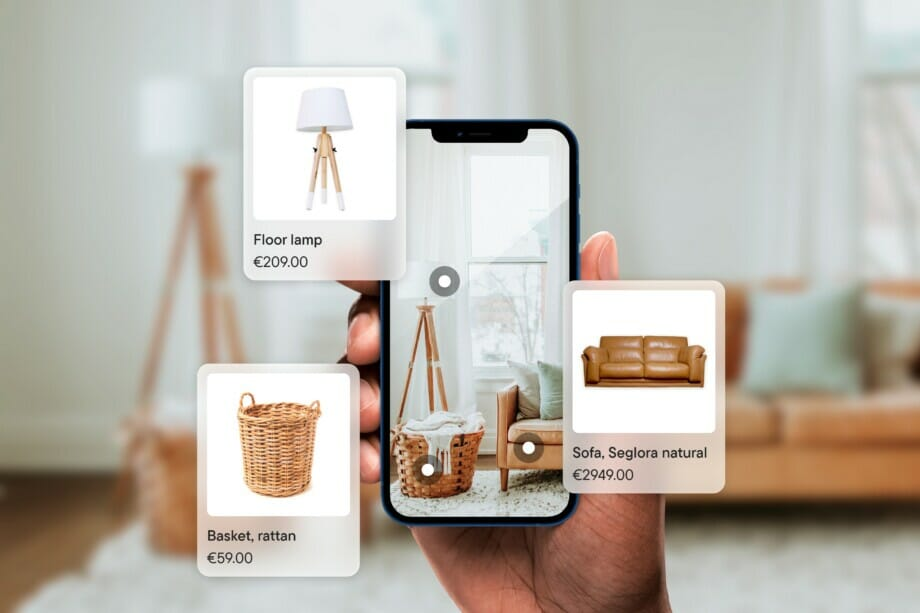
\includegraphics[height=7cm,width=12cm]{Chapitre1/img18.jpg}
          \caption{Shopping intelligent grâce à la détection d'objets.}
          \label{im18}
          \end{figure}

\section{Historique}
Au cours des deux dernières décennies, il est largement admis que les progrès de la détection d'objets ont généralement traversé deux périodes historiques : "\textbf{la période de détection d'objets traditionnelle (avant 2014)}" et "\textbf{la période de détection basée sur l'apprentissage profond (après 2014)}", comme le montre la figure \ref{histoire}

\begin{figure}[H]
\centering
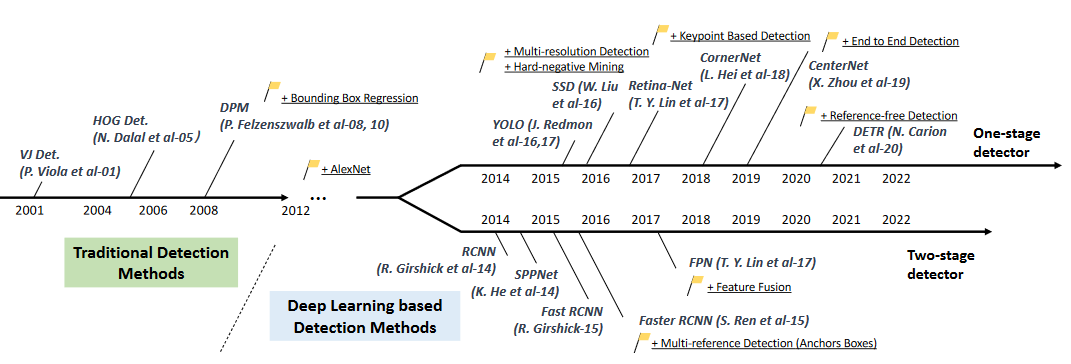
\includegraphics[height=8cm,width=17cm]{Chapitre1/histoire.png}
\caption{Timeline tiré de l'étude présentée par Zou et al. (2019) \cite{hist}.}
\label{histoire}
\end{figure}

\subsection{Période de détection d'objets traditionnels -Avant 2014-}
Dans cette période, la détection d'objets a été effectuée grâce à des techniques classiques d'apprentissage automatique. Parmi les plus remarquables des approches traditionnelles, on peut notamment citer :
 
\subsection{Le détecteur de Viola-Jones  (2001)}
C'est le travail pionnier qui a lancé le développement des méthodes traditionnelles de détection d'objets.

Il est originalement développé en 2001 par Paul Viola et Michael Jones \cite{violas} pour la détection de visages humains en temps réel, Il s'est également avéré utile dans d'autres applications.

Il utilise des fenêtres glissantes pour parcourir tous les emplacements et les  échelles possibles dans une image afin de vérifier si une fenêtre contient un visage humain. 

Les fenêtres glissante recherchent essentiellement des caractéristiques de Haar "Haar features"  (du nom d'Alfred Haar qui a développé le concept des ondelettes de Haar) (voir figure \ref{haar}).

\begin{figure}[H]
\centering
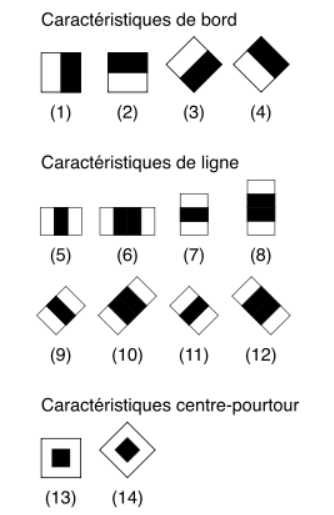
\includegraphics[height=7cm,width=7cm]{Chapitre1/haar.png}
\caption{Caractéristiques de Haar (Wikipédia).}
\label{haar}
\end{figure}

En outre, au lieu de simplement parcourir l'image avec une fenêtre glissante multi-échelles, ce qui est un processus très coûteux, les auteurs ont proposé trois techniques innovantes qui ont considérablement amélioré l'efficacité de l'approche :  

\begin{itemize}
\item Le calcul de l'intégrale de l'image, qui permet d'accélérer la convolution en recherchant dans un tableau dit des surfaces additionnées, des valeurs pré-calculées.
\item L'utilisation d'Adaboost, une méthode d'apprentissage itérative qui  utilise des arbres de décisions pour sélectionner les caractéristiques les plus pertinents.
\item La détection en cascade, qui est un moyen de combiner plusieurs classificateurs complexes en se concentrant progressivement sur le premier plan de l'image avec le plus d'informations.
\end{itemize}
    
\subsection{L'histogramme des gradients orientés  (2005)}

Proposé à l'origine en 2005 par N. Dalal et B. Triggs \cite{hog}, l'histogramme des gradients orientés (en anglais, histogram of oriented gradients ou HOG) est une amélioration des descripteurs SIFT, Shape contexts et les histogrammes d'orientation de contours. 

Le descripteur fournit une solution robuste invariante à l'échelle. 
Comme son nom l'indique, “HOG” calcule une carte des histogrammes des gradients de l'image, qui est ensuite pondérée par la moyenne des gradients d'images à partir de l'ensemble de données d'apprentissage.

La figure \ref{hog} montre une aperçu de la méthode HOG avec les histogrammes de gradients calculées localement et pondérées avec les exemples d'entraînement.

La méthode est largement connue pour son utilisation dans la détection des piétons. Pour détecter des objets de différentes tailles, et particulièrement pour la détection de personnes.

\begin{figure}[H]
\centering
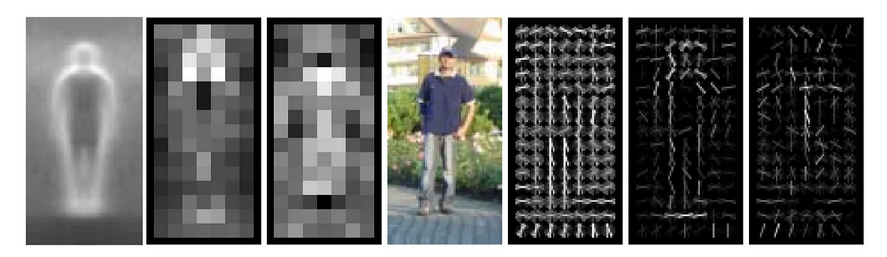
\includegraphics[height=6cm,width=17cm]{Chapitre1/hog.png}
\caption{Aperçu du descripteur HOG avec les histogrammes de gradients calculées localement et pondérées avec les exemples d'entraînement \cite{w1}.}
\label{hog}
\end{figure}


\subsection{Modèle partiel déformable (DPM) (2008)} 

Le modèle partiel déformable (DPM) \cite{dpm } a été proposé à l'origine par P. Felzenszwalb en 2008 comme une extension du détecteur HOG, mais qui introduit la stratégie de l'apprentissage des parties et de leur ensemble. 
Par exemple, le problème de la détection d'une « voiture » peut être décomposé en utilisant une stratégie de « diviser pour mieux régner » en détectant sa fenêtre, sa carrosserie et ses roues. Le processus d'entraînement implique l'apprentissage d'une manière appropriée de décomposer un objet, et l'inférence implique l'assemblage de détections de différentes parties d'objet.

La figure \ref{dpm}  montre un aperçu de la méthode DPM. A gauche, on voit la détection  DPM de deux personnes dans des poses différentes et à droite le modèle d'apprentissage basé sur l’histogramme des gradients de l'ensemble et des parties d'un humain.

\begin{figure}[H]
\centering
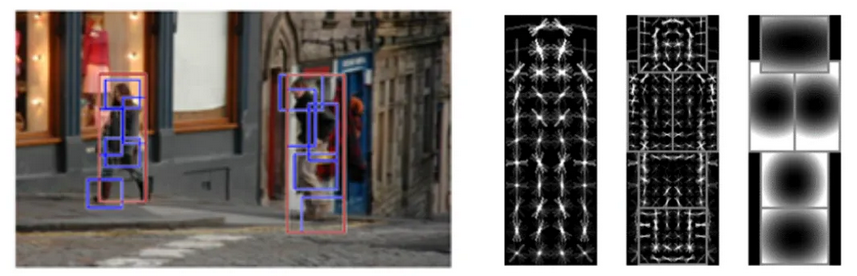
\includegraphics[height=6cm,width=17cm]{Chapitre1/dpm.png}
\caption{un aperçu de la méthode DPM \cite{w1}.}
\label{dpm}
\end{figure}

Bien que développé en 2008. Plus tard, une variété d'améliorations ont été apportées par R. Girshick, et il continue à inspirer des méthodes de détection jusqu'à présent.

     
\subsection{Période de Deep Learning Detection - Après 2014 –} 
Malgré le succès des approches classiques, l'effort requis pour créer des modèles de détection efficaces et efficients reste important. Par conséquent, Elles ont été complètement remplacées par des méthodes basées sur des réseaux de neurones profonds, ce qui se traduit par une plus grande précision et généralisation. À l'ère de l'apprentissage en profondeur, la détection d'objets est regroupée en deux classes : la "détection en deux étapes" et la "détection en une étape".

Les principaux algorithmes de détection d'objets en deux étapes sont:

    \begin{itemize}
    \item RCNN and SPPNet (2014)
    \item Fast RCNN and Faster RCNN (2015)
    \item Mask R-CNN (2017)
    \item Pyramid Networks/FPN (2017)
    \item G-RCNN (2021)
    \end{itemize}
    
Les principaux algorithmes de détection d'objets en une seule étape sont :

    \begin{itemize}
    \item YOLO (2016)
    \item SSD (2016)
    \item RetinaNet (2017)
    \item YOLOv3 (2018)
    \item YOLOv4 (2020)
    \item YOLOR (2021)
    \item YOLOv7 (2022)
    \end{itemize}
     

\section{Conclusion}
Nous avons défini ce qu'est la détection d'objets et nous l'avons distinguée des autres tâches de vision par ordinateur.

Nous avons mentionné quelques cas d'utilisation de la détection d'objets et nous avons parlé de l'histoire de la détection d'objets et de ses 2 phases : avant l'apprentissage en profondeur et après l'apprentissage en profondeur.

